\section{Auswertung}
\label{sec:Auswertung}

Für die Auswertung wird Python und im Speziellen
Matplotlib \cite{matplotlib}, SciPy \cite{scipy},
Uncertainties \cite{uncertainties} und NumPy \cite{numpy} verwendet.

\noindent Die Werte für die Abstände in Abb. \ref{fig:Strahlgeometrie} sind
\begin{align*}
    x_0 &= \SI{83}{\milli\meter} \\
    x_1 &= \SI{67}{\milli\meter} \\
    x_2 &= \SI{100}{\milli\meter}.
\end{align*}
Die mit Gleichung \eqref{eqn:V} ermittelten Luftvolumina
für die Blendendurchmesser $d_1 = \SI{2}{\milli\meter}$ und
$d_2 = \SI{5}{\milli\meter}$ sind
\begin{align*}
    V_1 &= \SI{27.77}{\centi\meter\cubed} \\ 
    V_2 &= \SI{173.5}{\centi\meter\cubed}.  
\end{align*}


\subsection{Bestimmung der Ionendosisrate und der Energiedosisrate}

%Ionendosis J aus V und I_S bestimmen
Der Kondensatorstrom $I_\text{K}$ in Abhängigkeit von der
Kondensatorspannung $U_\text{K}$ bei der Blende mit
$d_1 = \SI{2}{\milli\meter}$ ist in Tab. \ref{taba} und in Fig. \ref{plota}
dargestellt. Die Werte für die Blende mit 
$d_2 = \SI{5}{\milli\meter}$ befinden sich in Tab. \ref{tabb} und sind in 
Fig. \ref{plotb} dargestellt worden.

\begin{table}\caption{Die Länge der Zylinder und die Spannung mit den jeweiligen Zeitenpunkten der Ausschläge.}
\label{taba}
\centering
\sisetup{round-mode = places, round-precision=2, round-integer-to-decimal=true}
\begin{tabular}{S[]S[]S[]S[]S[]} 
\toprule
{$l/ \si{\milli\meter}$} & {$U_1/ \si{\volt}$} & {$t_1/ \si{\micro\second}$} & {$U_2/ \si{\volt}$} & {$t_2/ \si{\micro\second}$}\\
\midrule
120.8 & 1.29 & 0.6 & 0.17 & 88.7\\
102.3 & 1.27 & 0.5 & 0.2 & 76.5\\
80.5 & 1.33 & 0.6 & 0.76 & 59.8\\
40.4 & 1.33 & 0.5 & 1.34 & 30.2\\
31.1 & 1.29 & 0.5 & 1.37 & 23.8\\
\bottomrule
\end{tabular}\end{table}
\begin{table}\caption{Die angelegte Spannung des elektrischen Feldes innerhalb des Geiger-Müller-Zählrohrs, die Anzahl der jeweils gemessenen Impulse und der Strom innerhalb des Geiger-Müller-Zählrohrs.}
\label{tabb}
\centering
\sisetup{round-mode = places, round-precision=2, round-integer-to-decimal=true}
\begin{tabular}{c c S[]} 
\toprule
{$U / \si{\volt}$} & {$\frac{N}{\SI{130}{\second}}$} & {$I / \si{\ampere}$}\\
\midrule
320 & 11298 & 0.1\\
400 & 11820 & 0.2\\
480 & 12135 & 0.3\\
540 & 12301 & 0.35\\
560 & 12068 & 0.4\\
600 & 12354 & 0.45\\
640 & 12403 & 0.5\\
660 & 12507 & 0.55\\
680 & 12659 & 0.6\\
\bottomrule
\end{tabular}\end{table}

\begin{figure}
    \centering
    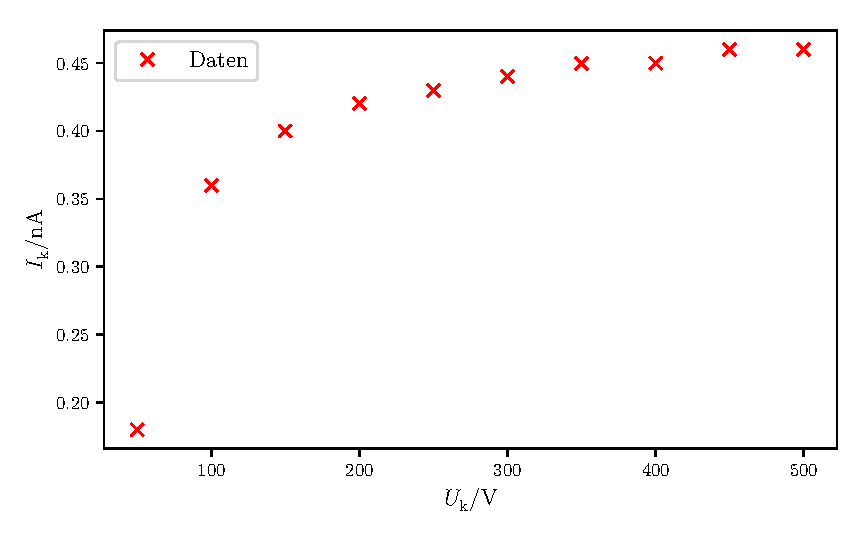
\includegraphics[width=15cm, height=9cm]{build/plota.pdf}
    \caption{Die Kathodenspannung $U_\text{K}$ und der Kathodenstrom $I_\text{K}$ sind in diesem Plot gegeneinander aufgetragen. Die Beschleunigungsspannung $U_\text{B}$ beträgt $\SI{25}{\kilo\volt}$, der Anodenstrom $I_\text{A}$ beträgt $\SI{1}{\milli\ampere}$. Der Blendendurchmesser beträgt $\SI{2}{\milli\meter}$.}
    \label{plota}
\end{figure}

\begin{figure}
    \centering
    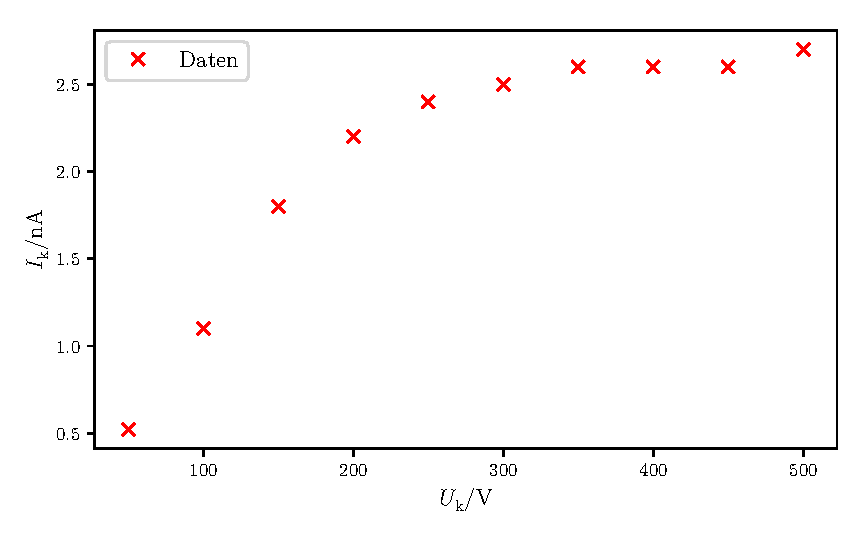
\includegraphics[width=15cm, height=9cm]{build/plotb.pdf}
    \caption{Die Kathodenspannung $U_\text{K}$ und der Kathodenstrom $I_\text{K}$ sind in diesem Plot gegeneinander aufgetragen. Die Beschleunigungsspannung $U_\text{B}$ beträgt $\SI{25}{\kilo\volt}$, der Anodenstrom $I_\text{A}$ beträgt $\SI{1}{\milli\ampere}$. Der Blendendurchmesser beträgt $\SI{5}{\milli\meter}$.}
    \label{plotb}
\end{figure}

\noindent Aus den Sättigungswerten des Kondensatorstroms ergibt sich die Ionendosisrate $\dot{J}$ und die Energiedosisrate $\dot{D}$. 
Der Sättigungswert für die kleine Blende ergibt sich zu 
\begin{equation*}
    I_\text{Sättigung, 1} = \SI{0.45}{\nano\ampere}.
\end{equation*}
Für die große Blende ergibt sich ein Wert von 
\begin{equation*}
    I_\text{Sättigung, 2} = \SI{2.6}{\nano\ampere}.
\end{equation*}

\noindent Somit lässt sich die Ionendosisrate mit Gleichung \eqref{eqn:Ionendosisrate} als die Werte  
\begin{align*}
    \dot{J}_\text{1} &= \SI{1.344e-5}{\ampere\per\kilo\gram}\\
    \dot{J}_\text{2} &= \SI{1.245e-5}{\ampere\per\kilo\gram} 
\end{align*}
bestimmen.

\noindent Der Mittelwert ergibt sich damit zu 
\begin{equation*}
    \dot{J}_\text{mittel} = \SI{1.29(05)e-5}{\ampere\per\kilo\gram}.
\end{equation*}

\noindent Die Anzahl der erzeugten Ionen ergibt sich mit Gleichung \eqref{eqn:Ionenanzahl} zu 
\begin{equation*}
    n = \SI{8.09(31)e13}{\per\kilo\gram\per\second}.
\end{equation*}

%mit Ionisationsenergie eines Luftmoleküls (Wert R aus Anleitung?) Energiedosis D und Energiedosisrate D° berechnen
\noindent Mit dem Wert \cite{Luft} von 
\begin{equation*}
    \Phi_\text{Luft} = \SI{33}{\electronvolt} = \SI{52.8e-19}{\joule}
\end{equation*}
ergibt sich die mittlere Energiedosisrate von 
\begin{equation*}
    \dot{D}_\text{m} = \SI{4.27(16)e-4}{\joule\per\kilo\gram\per\second}.
\end{equation*}



\subsection{Ionenstrom als Funktion des Anodenstroms}

Die Kondensatorströme $I_\text{K}$ in Abhängigkeit vom
Anodenstrom $I_\text{A}$ für die beiden Kondensatorspannungen
$U_\text{K, 1} = \SI{500}{\volt}$ und $U_\text{K, 2} = \SI{300}{\volt}$
sind in Tab. \ref{tabc} eingetragen.

\subsubsection{Erste Kondensatorspannung}
%I_K gegen I_A plotten
Die $I_\text{K}$- und $I_\text{A}$-Werte stehen in Tab. \ref{tabc} und sind in Abb. \ref{fig:plot1} aufgetragen. 

\begin{table}\caption{Der Anodenstrom und der Kathodenstrom bei einer Beschleunigungsspannung von $U_\text{B} = \SI{25}{\kilo\volt}$ und einer Kathodenspannung $U_\text{K,1} = \SI{500}{\volt}$ und einer Kathodenspannung $U_\text{K,2} = \SI{300}{\volt}$ bei einem Blendenradius von $r_\text{B} = \SI{5}{\milli\meter}$.}
\label{tabc}
\centering
\sisetup{round-mode = places, round-precision=2, round-integer-to-decimal=true}
\begin{tabular}{S[]S[]S[]} 
\toprule
{$I_\text{K} / \si{\milli\ampere}$} & {$I_\text{K,1} / \si{\nano\ampere}$} & {$I_\text{K,2} / \si{\nano\ampere}$}\\
\midrule
1.0 & 2.6 & 2.4\\
0.95 & 2.5 & 2.4\\
0.9 & 2.4 & 2.2\\
0.85 & 2.3 & 2.1\\
0.8 & 2.2 & 2.0\\
0.75 & 2.1 & 1.9\\
0.7 & 1.9 & 1.8\\
0.65 & 1.8 & 1.6\\
0.6 & 1.6 & 1.5\\
0.55 & 1.5 & 1.4\\
0.5 & 1.4 & 1.3\\
0.45 & 1.2 & 1.2\\
0.4 & 1.1 & 1.0\\
0.35 & 0.9 & 0.9\\
0.3 & 0.8 & 0.8\\
0.25 & 0.6 & 0.6\\
0.2 & 0.5 & 0.5\\
0.15 & 0.4 & 0.4\\
0.1 & 0.1 & 0.2\\
0.05 & 0.1 & 0.1\\
\bottomrule
\end{tabular}\end{table}

\begin{figure}
    \centering
    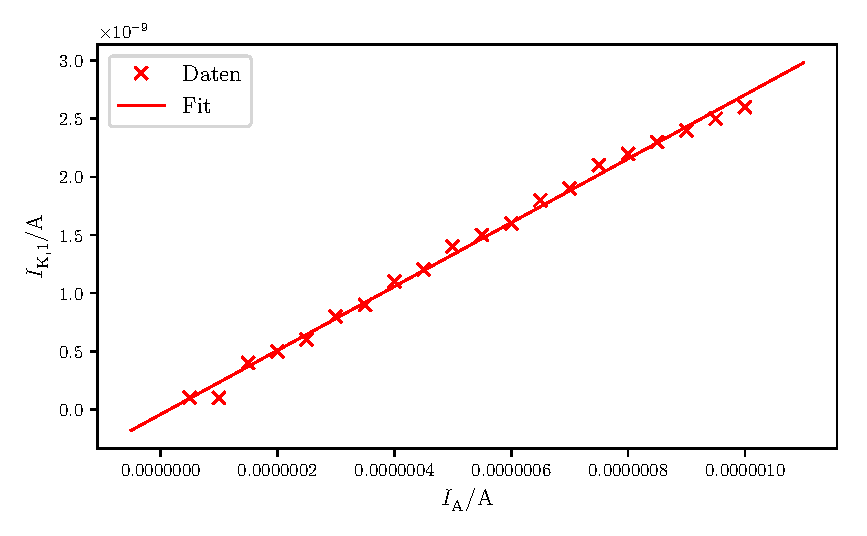
\includegraphics[width=15cm, height=9cm]{build/plot1.pdf}
    \caption{Der Kathodenstrom $I_\text{K}$ und der Anodenstrom $I_\text{A}$ sind gegeneinander aufgetragen. Die Beschleunigungsspannung $U_\text{B}$ beträgt $\SI{25}{\kilo\volt}$. Die Kathodenspannung $U_\text{K}$ beträgt ,$\SI{500}{\volt}$. Der Blendendurchmesser ist $\SI{5}{\milli\meter}.$}
    \label{fig:plot1}
\end{figure}

\noindent Die Parameter, die sich aus der linearen Regression nach Gleichung \eqref{eqn:linreg} ergeben, betragen
\begin{align*}
    a &= \num{27.48(04)e-4}\\
    b &= \SI{-4.32e-11}{\ampere},
\end{align*}
wobei $a$ die Steigung und $b$ der $y$-Achsenabschnitt ist. 

\subsubsection{Zweite Kondensatorspannung}
%I_K gegen I_A plotten
Die $I_\text{K}$- und $I_\text{A}$-Werte stehen in Tab. \ref{tabc} und sind in Abb. \ref{fig:plot2} aufgetragen. 

\begin{figure}
    \centering
    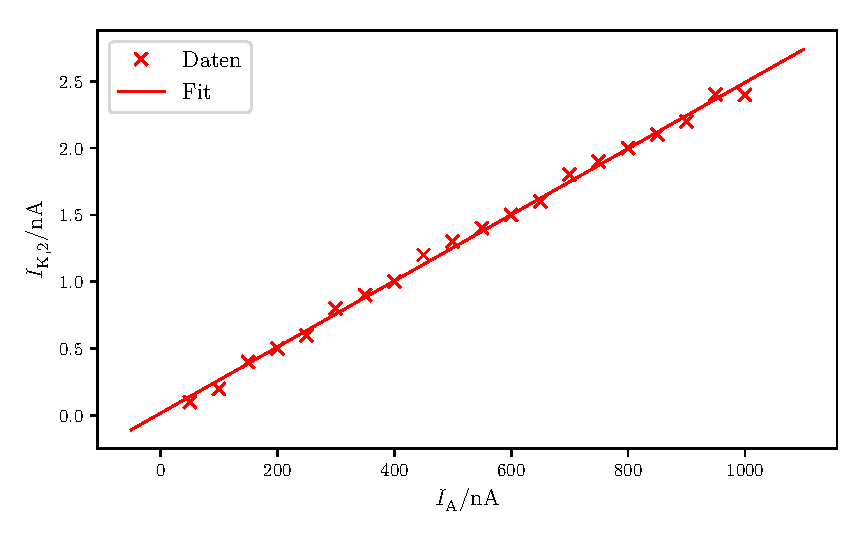
\includegraphics[width=15cm, height=9cm]{build/plot2.pdf}
    \caption{Der Kathodenstrom $I_\text{K}$ und der Anodenstrom $I_\text{A}$ sind gegeneinander aufgetragen. Die Beschleunigungsspannung $U_\text{B}$ beträgt $\SI{25}{\kilo\volt}$. Die Kathodenspannung $U_\text{K}$ beträgt ,$\SI{300}{\volt}$. Der Blendendurchmesser ist $\SI{5}{\milli\meter}.$}
    \label{fig:plot2}
\end{figure}

\noindent Die Parameter, die sich aus der linearen Regression nach Gleichung \eqref{eqn:linreg} ergeben, betragen
\begin{align*}
    a &= \num{24.74(03)e-4}\\
    b &= \SI{-1.63e-11}{\ampere},
\end{align*}
wobei $a$ die Steigung und $b$ der $y$-Achsenabschnitt ist. 



\subsection{Ionenstrom als Funktion der Beschleunigungsspannung}

Die Kondensatorströme $I_\text{K}$ in Abhängigkeit von der
Beschleunigungsspannung $U_\text{B}$ für die beiden Kondensatorspannungen
$U_\text{K, 1} = \SI{500}{\volt}$ und $U_\text{K, 2} = \SI{300}{\volt}$
sind in Tab. \ref{tabd} eingetragen.

\subsubsection{Erste Kondensatorspannung}
%I_K gegen U_B plotten
Die $I_\text{K}$- und $U_\text{B}$-Werte stehen in Tab. \ref{tabd} und sind in Abb. \ref{fig:plot3} aufgetragen. 

\begin{table}\caption{Laufzeiten und Spannungen der reflektierten Impulse bei dem Modell des Auges.}
\label{tabd}
\centering
\sisetup{round-mode = places, round-precision=2, round-integer-to-decimal=true}
\begin{tabular}{S[]S[]} 
\toprule
{$t_1/ \si{\micro\second}$} & {$U_1/ \si{\volt}$}\\
\midrule
1.0 & 1.38\\
11.7 & 1.0\\
16.1 & 1.25\\
22.9 & 0.95\\
72.2 & 0.4\\
\bottomrule
\end{tabular}\end{table}

\begin{figure}
    \centering
    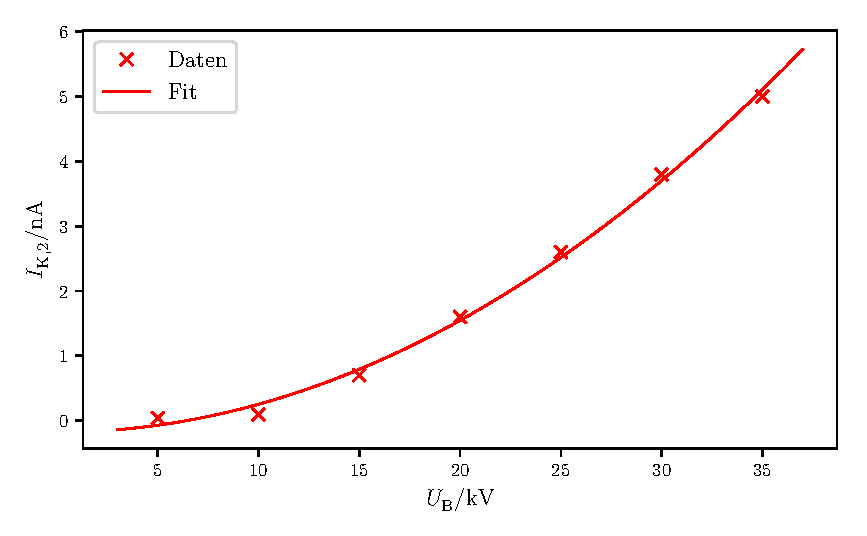
\includegraphics[width=15cm, height=9cm]{build/plot3.pdf}
    \caption{Der Kathodenstrom $I_\text{K}$ und die Beschleunigungsspannung $U_\text{B}$ sind gegeneinander aufgetragen. Der Anodenstrom $I_\text{A}$ beträgt $\SI{1}{\milli\ampere}$. Die Kathodenspannung $U_\text{K}$ beträgt ,$\SI{500}{\volt}$. Der Blendendurchmesser ist $\SI{5}{\milli\meter}.$}
    \label{fig:plot3}
\end{figure}

\noindent Die Parameter, die sich aus der Ausgleichsrechnung nach Gleichung \eqref{eqn:quadreg} ergeben, betragen
\begin{align*}
    a &= \SI{4.314(112)e-18}{\ampere\per\volt}\\
    b &= \SI{-1.8(7)e-10}{\ampere},
\end{align*}
wobei $a$ die Amplitude und $b$ der $y$-Achsenabschnitt ist. 

\subsubsection{Zweite Kondensatorspannung}
%I_K gegen U_B plotten
Die $I_\text{K}$- und $U_\text{B}$-Werte stehen in Tab. \ref{tabd} und sind in Abb. \ref{fig:plot4} aufgetragen. 

\begin{figure}
    \centering
    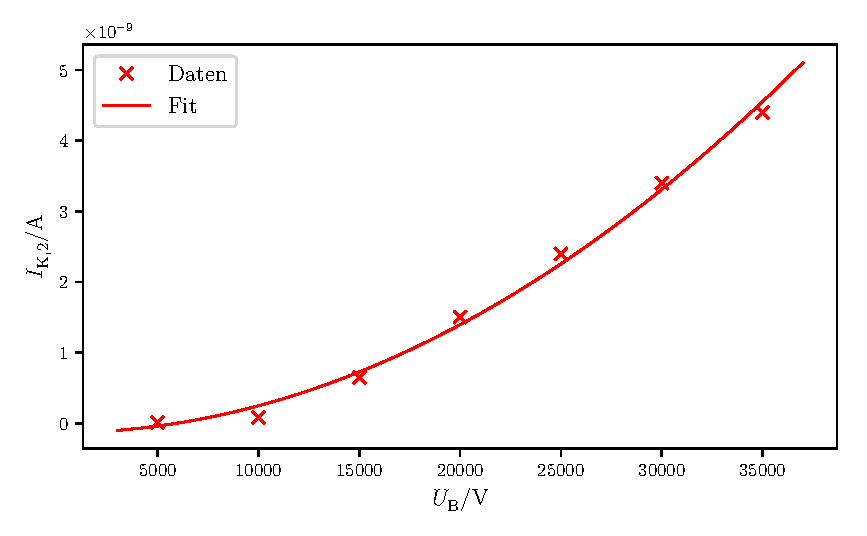
\includegraphics[width=15cm, height=9cm]{build/plot4.pdf}
    \caption{Der Kathodenstrom $I_\text{K}$ und die Beschleunigungsspannung $U_\text{B}$ sind gegeneinander aufgetragen. Der Anodenstrom $I_\text{A}$ beträgt $\SI{1}{\milli\ampere}$. Die Kathodenspannung $U_\text{K}$ beträgt ,$\SI{300}{\volt}$. Der Blendendurchmesser ist $\SI{5}{\milli\meter}.$}
    \label{fig:plot4}
\end{figure}

\noindent Die Parameter, die sich aus der Ausgleichsrechnung nach Gleichung \eqref{eqn:quadreg} ergeben, betragen
\begin{align*}
    a &= \SI{3.825(130)e-18}{\ampere\per\volt}\\
    b &= \SI{-1.35(8)e-10}{\ampere},
\end{align*}
wobei $a$ die Amplitude und $b$ der $y$-Achsenabschnitt ist.
